\section*{\texorpdfstring{Discrepancy in $\T$ between \s\ and \f\ GRBs}{}}
In Figure \ref{fig:T90_comparison} of Section \ref{sec:selecting_common_GRBs}, it was noted that some GRBs have systematically smaller $\T$ in \f\ than \s. Hence, Figure \ref{fig:T90_comparison} was re-plotted as Figure \ref{fig:T90_vs_T90}, with the traditional demarcation lines of `long' and `short' GRBs clearly indicated, to aid the eye. It is observed that for $11$ GRBs, the ratio between the \f\ and \s\ $\T$s is significantly different from unity. A question arises naturally: Is there any systematic effect of the way these instruments detect GRBs, for example their waveband and sensitivities to different redshifts? Does the way the different classes of GRB evolve also play a role in introducing this discrepancy? Or are we actually looking at a different, the so-called `intermediate' class, of GRBs? In this section, I will report ongoing and future work to answer these questions.

\begin{figure}
\begin{center}
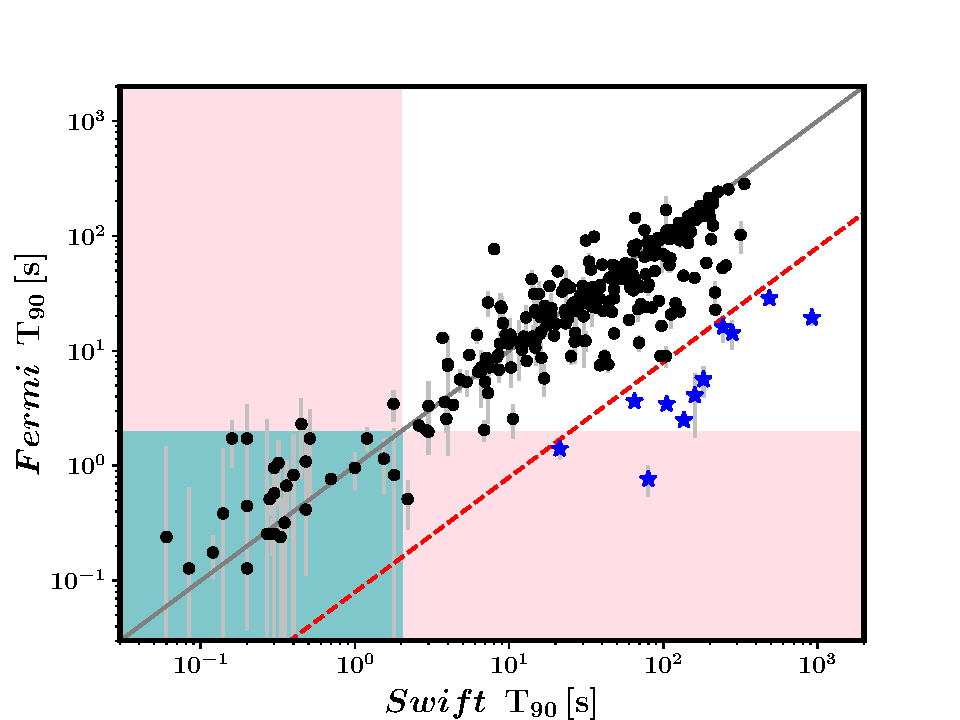
\includegraphics[scale=0.5]{T90_vs_T90--all}
\caption[Detailed comparison of $\T$s of \f\ and \s\ GRBs]{For the $265$ GRBs detected with both \s\ and \f\ in the $\sim 9$ years of operation. The green patch shows those which are ``short'' [$2$ s criterion] in both, the pink patches show those which are long in one but short in the other. The gray line is what would happen in the ideal world: the $\T$s would be equal. It is observed that systematically more number of GRBs have smaller $\T$ for \f\ than \s. In fact, if a cut of $10$ is placed on the ratio motivated by one GRB which is certainly long in \s\ while short in \f, it is seen that $11$ GRBs fall below that line.}
\label{fig:T90_vs_T90}
\end{center}
\end{figure}

First I confirmed that there are GCNs reporting the detection of all of the $11$ GRBs for both \f -GBM and the \s -BAT. Then I looked for reports in the literature which mention any of these GRBs in particular. There is no published paper reporting detailed analysis of $10$ out of $11$ of these GRBs, the exception being GRB 080928 [\s\ nomenclature] / GRB080928628 [\f\ nomenclature].

There are three papers mentioning this GRB, however, two of the latter papers [chronologically] actually mention the earliest \citep{Rossi_et_al.-2011-A&A}, quoting its results to put that in respective theoretical perspectives. That is because this earlier paper makes a decisive statement that this GRB is actually very peculiar: It had already started emitting its ``afterglow'' emission in the optical wavelengths while still giving out ``prompt'' emission in the gamma rays. In fact, it was first detected by the $\s$-BAT and discovered by \f -GBM $204$ s after the \s\ trigger, as demonstrated in their Figure 1 and Equation 1. It appears from their Figure 1 that the main burst happened after $204$ s of the first BAT detection [discounting the $-90$ s ``precursor'']. From a quick-look at the simultaneous \s\ BAT/XRT lightcurves\footnote{\url{http://www.swift.ac.uk/burst_analyser/}}, it is clear that the two instruments see the rising part of the flare for the main burst that $\f$ also sees. But this raises a question: What about the XRT data before that? Can it be established that these flares were intrinsically soft and hence \f\ did not see them? If that is indeed the case, why does the XRT flare coincide with the \f\ flare? Is it possible to have lower energy flares preceding higher energy ones? These mysteries are being currently investigated with a careful spectro-temporal analysis.

Looking at the common catalogue data shows that except this GRB, the difference in the trigger times for the two detectors is in most cases consistent with $0$, in a few cases going up to maximum of $4$ s. A thorough manual check in the data for the common catalogue, as well as the original data files used for creating this catalogue validates the time difference for each of these $10$ GRBs. This indeed throws up a mystery: What is happening to these GRBs? Are they systematically softer so that \f, which calculates the $\T$ in the $50$-$300$ keV waveband instead of $\s$'s $15$-$150$ keV waveband, measures systematically smaller $\T$? If that is indeed the case, then can a energy-dependent analysis of the observed $\T$ be made? Or are we looking at a strange class of `intermediate' GRBs \citep{Horvath_&_Toth-2016-Ap&SS}? The best way forward is to create \f -GBM and \s\ lightcurves, both BAT and XRT, and compare the emission across the wavelengths. This is currently being attempted one GRB at a time. Quick-look lightcurves of \s, both BAT and XRT, have been obtained for all the $11$ GRBs from \href{http://www.swift.ac.uk/burst_analyser/}{the Swift Quick-Look Website}, and the idea is that in most cases, \s -BAT sees not only the prompt emission, but also the afterglow emission, because it observes at a softer band than \f -GBM. If this fact could be established, it would imply that the $\T$s reported by \s\ by an automated analysis are incorrect for these bursts. This would then require careful modification of the automatic analysis software to infer this number, because the $\T$influences the way the other bursts properties, like the total energy output, are calculated. It is envisaged that a concrete result will be produced in around $6$ months from now.